\documentclass{scrartcl}
\usepackage[mathletters]{ucs}
\usepackage[utf8x]{inputenc}
\usepackage{amssymb}
\usepackage{amsmath}
\usepackage[usenames]{color}
\usepackage{hyperref}
\usepackage{wasysym}
\usepackage{graphicx}
\usepackage[normalem]{ulem}
\usepackage{enumerate}

\usepackage{listings}

\lstset{ %
basicstyle=\footnotesize,       % the size of the fonts that are used for the code
showspaces=false,               % show spaces adding particular underscores
showstringspaces=false,         % underline spaces within strings
showtabs=false,                 % show tabs within strings adding particular underscores
frame=single,                   % adds a frame around the code
tabsize=2,                      % sets default tabsize to 2 spaces
breaklines=true,                % sets automatic line breaking
breakatwhitespace=false,        % sets if automatic breaks should only happen at whitespace
}


\title{first wheel holder}
\date{dinsdag 08 december 2020}
\author{}

\begin{document}

\maketitle

		\section{first wheel holder}

Created vrijdag 13 november 2020



To be able to quickly create a lot of photos in a consistant way, a wheel is designed to mount 20 tools at once; using a stepper motor and a fixed camera and lighting setup the process of taking images would be automated for every 20 tools. The holder will be 3D printed so a few wheels can be made to be able to swap the wheels with new tools for an efficient dataset creation.



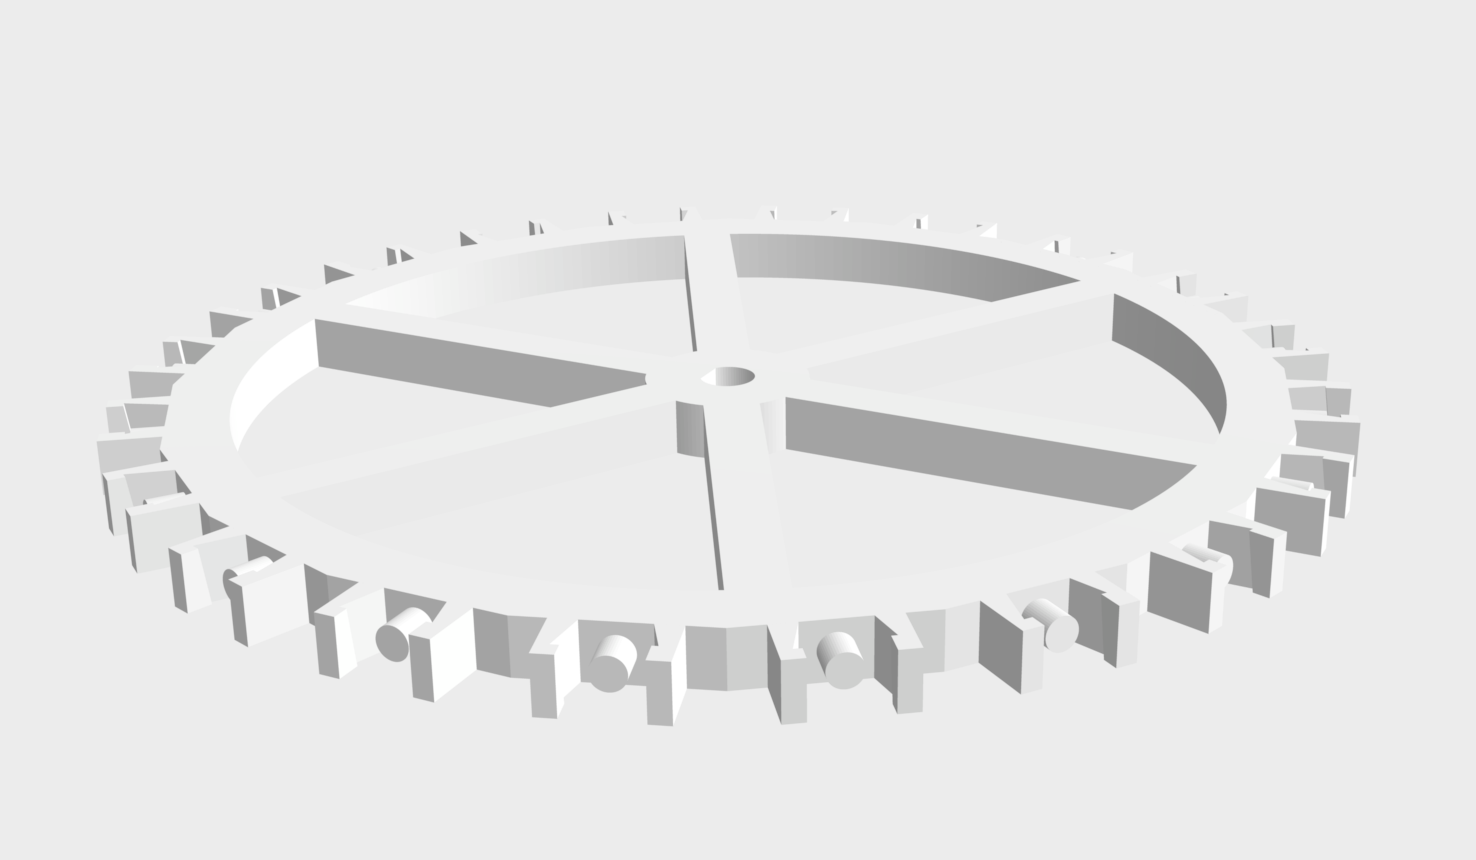
\includegraphics[height=3.125000in, keepaspectratio=true]{./first_wheel_holder/radhouder.png}



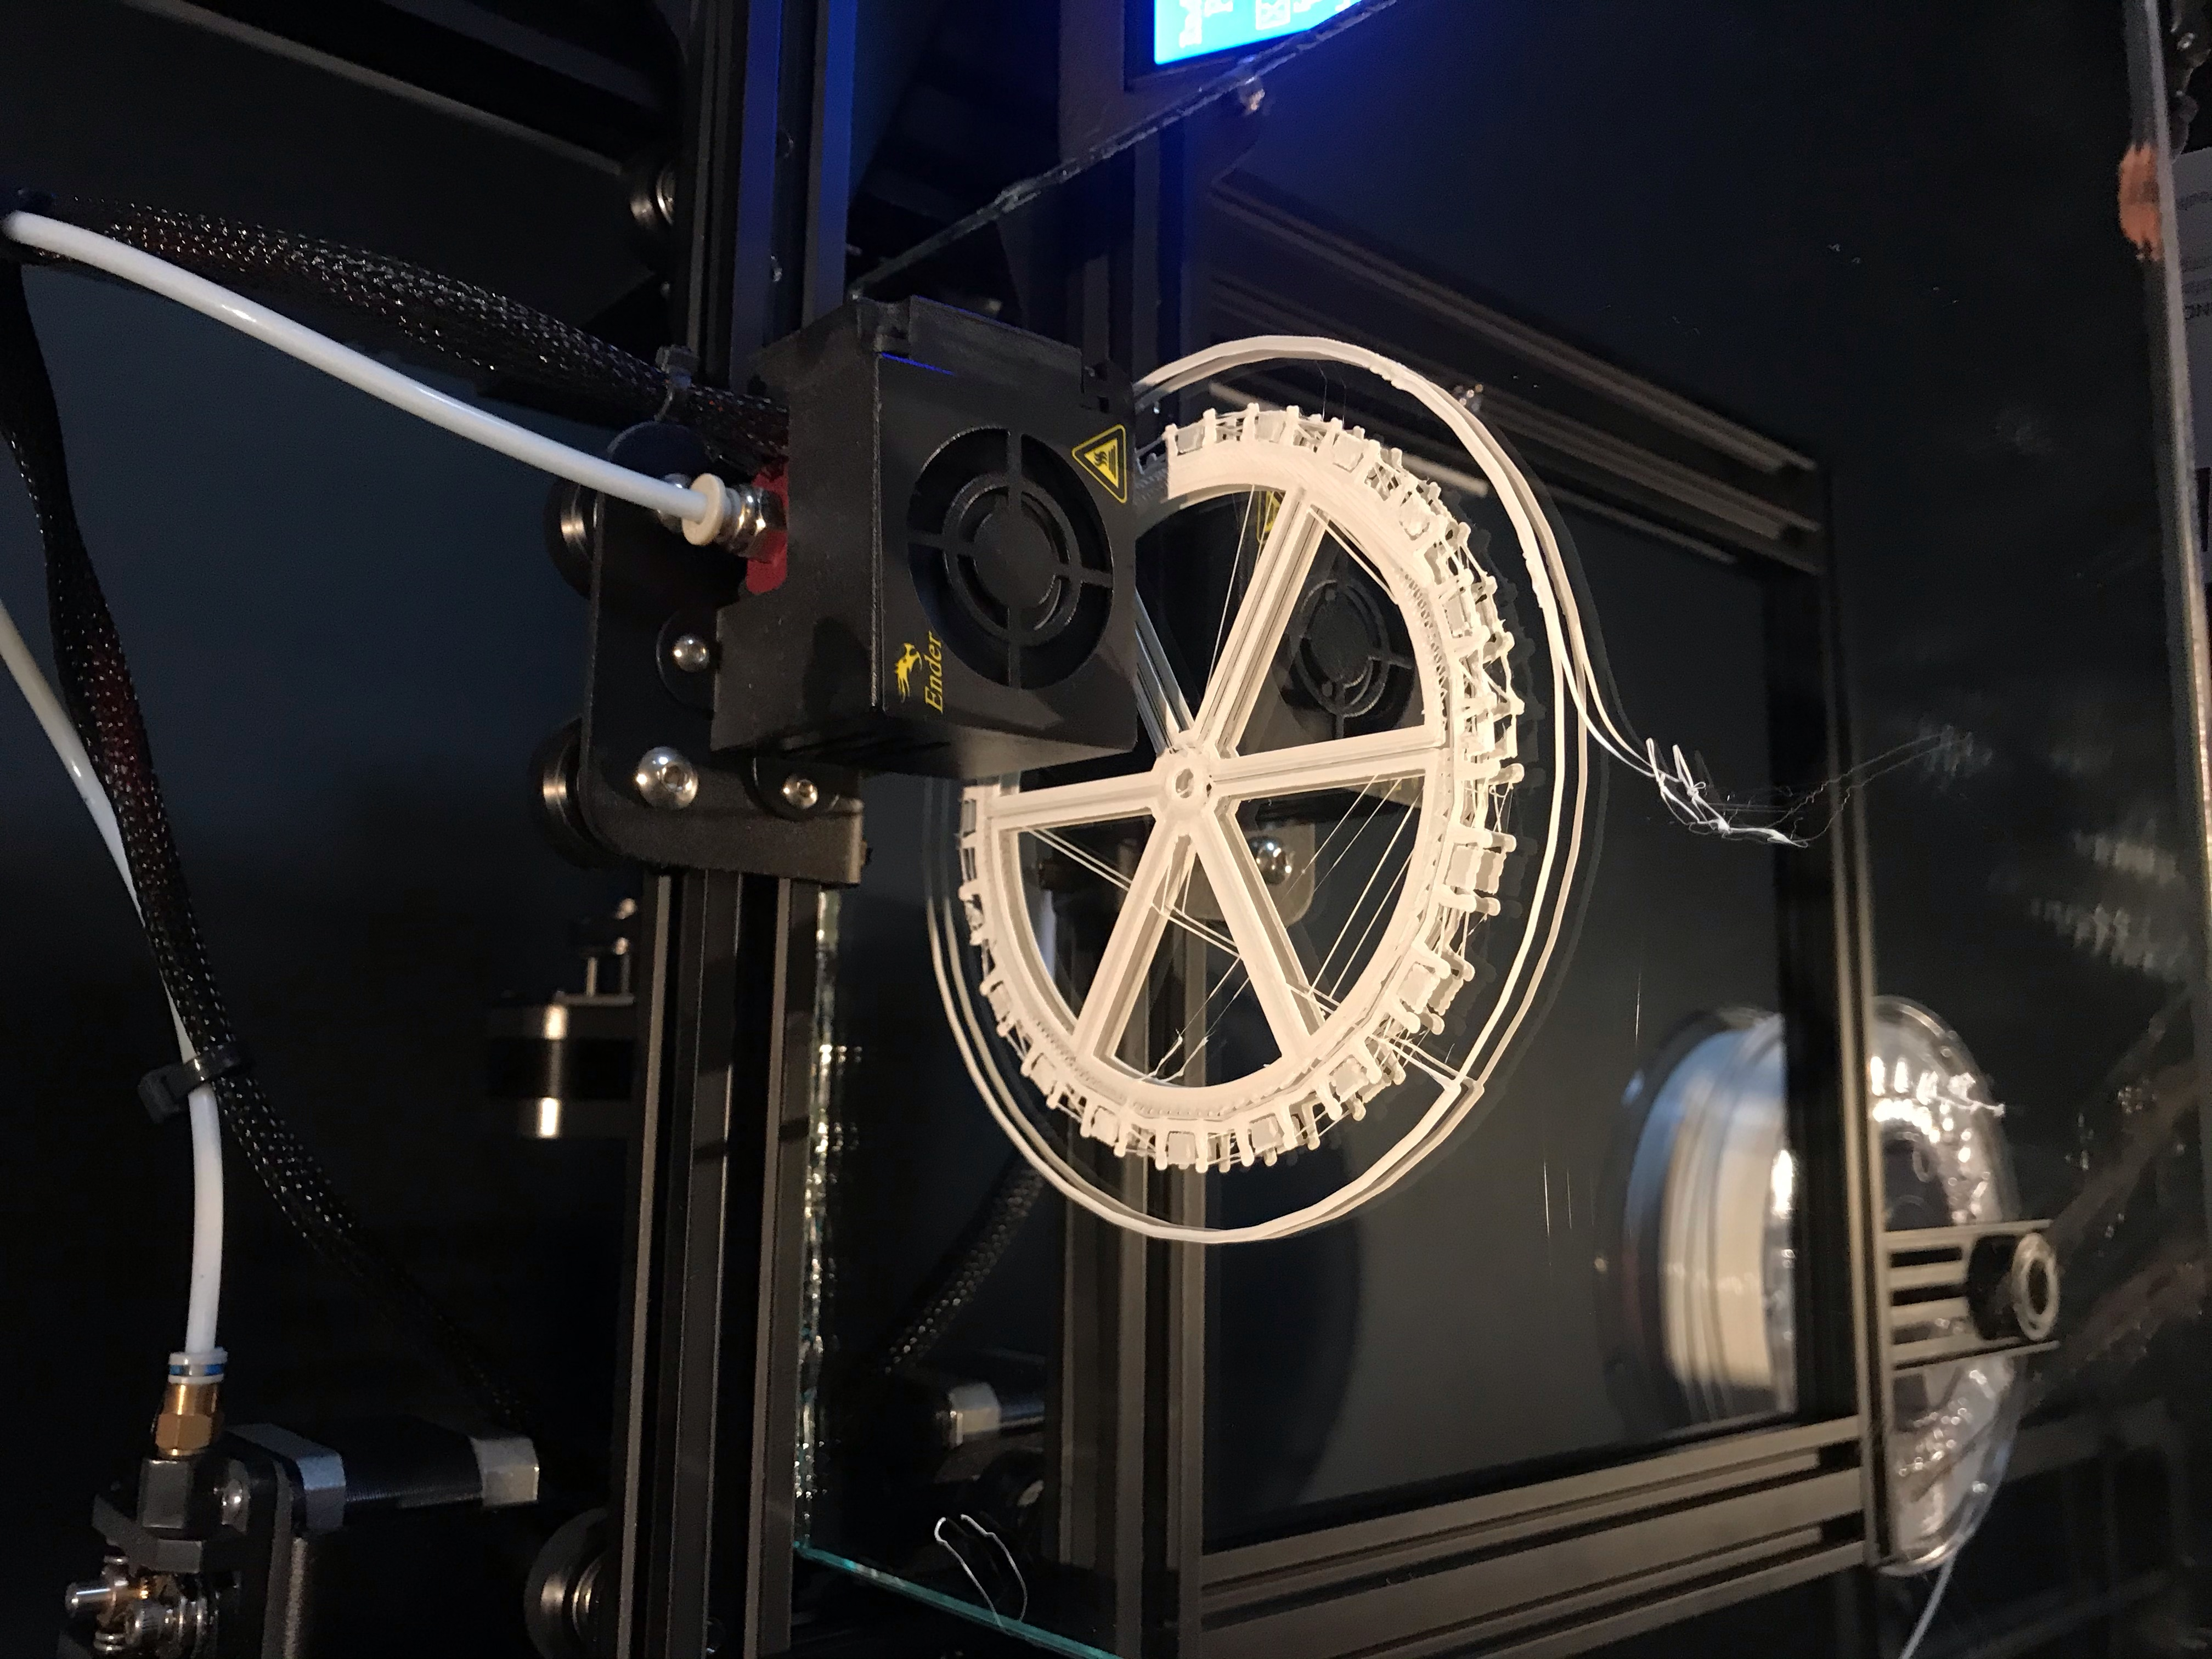
\includegraphics[height=3.125000in, keepaspectratio=true]{./first_wheel_holder/radhouder_duringprint.jpeg}

After printing the wheel had to be cleared from rest pieces of plastic and had to be tested with a tool, this made it possible to scratch the tool extra hard which would mean the given labels for that tool aren't correct anymore. The tool used is from 3 number 6 36*. the manual removal also means the tools dont sit in the same position in every place on the wheel. This will show in the generated pictures.

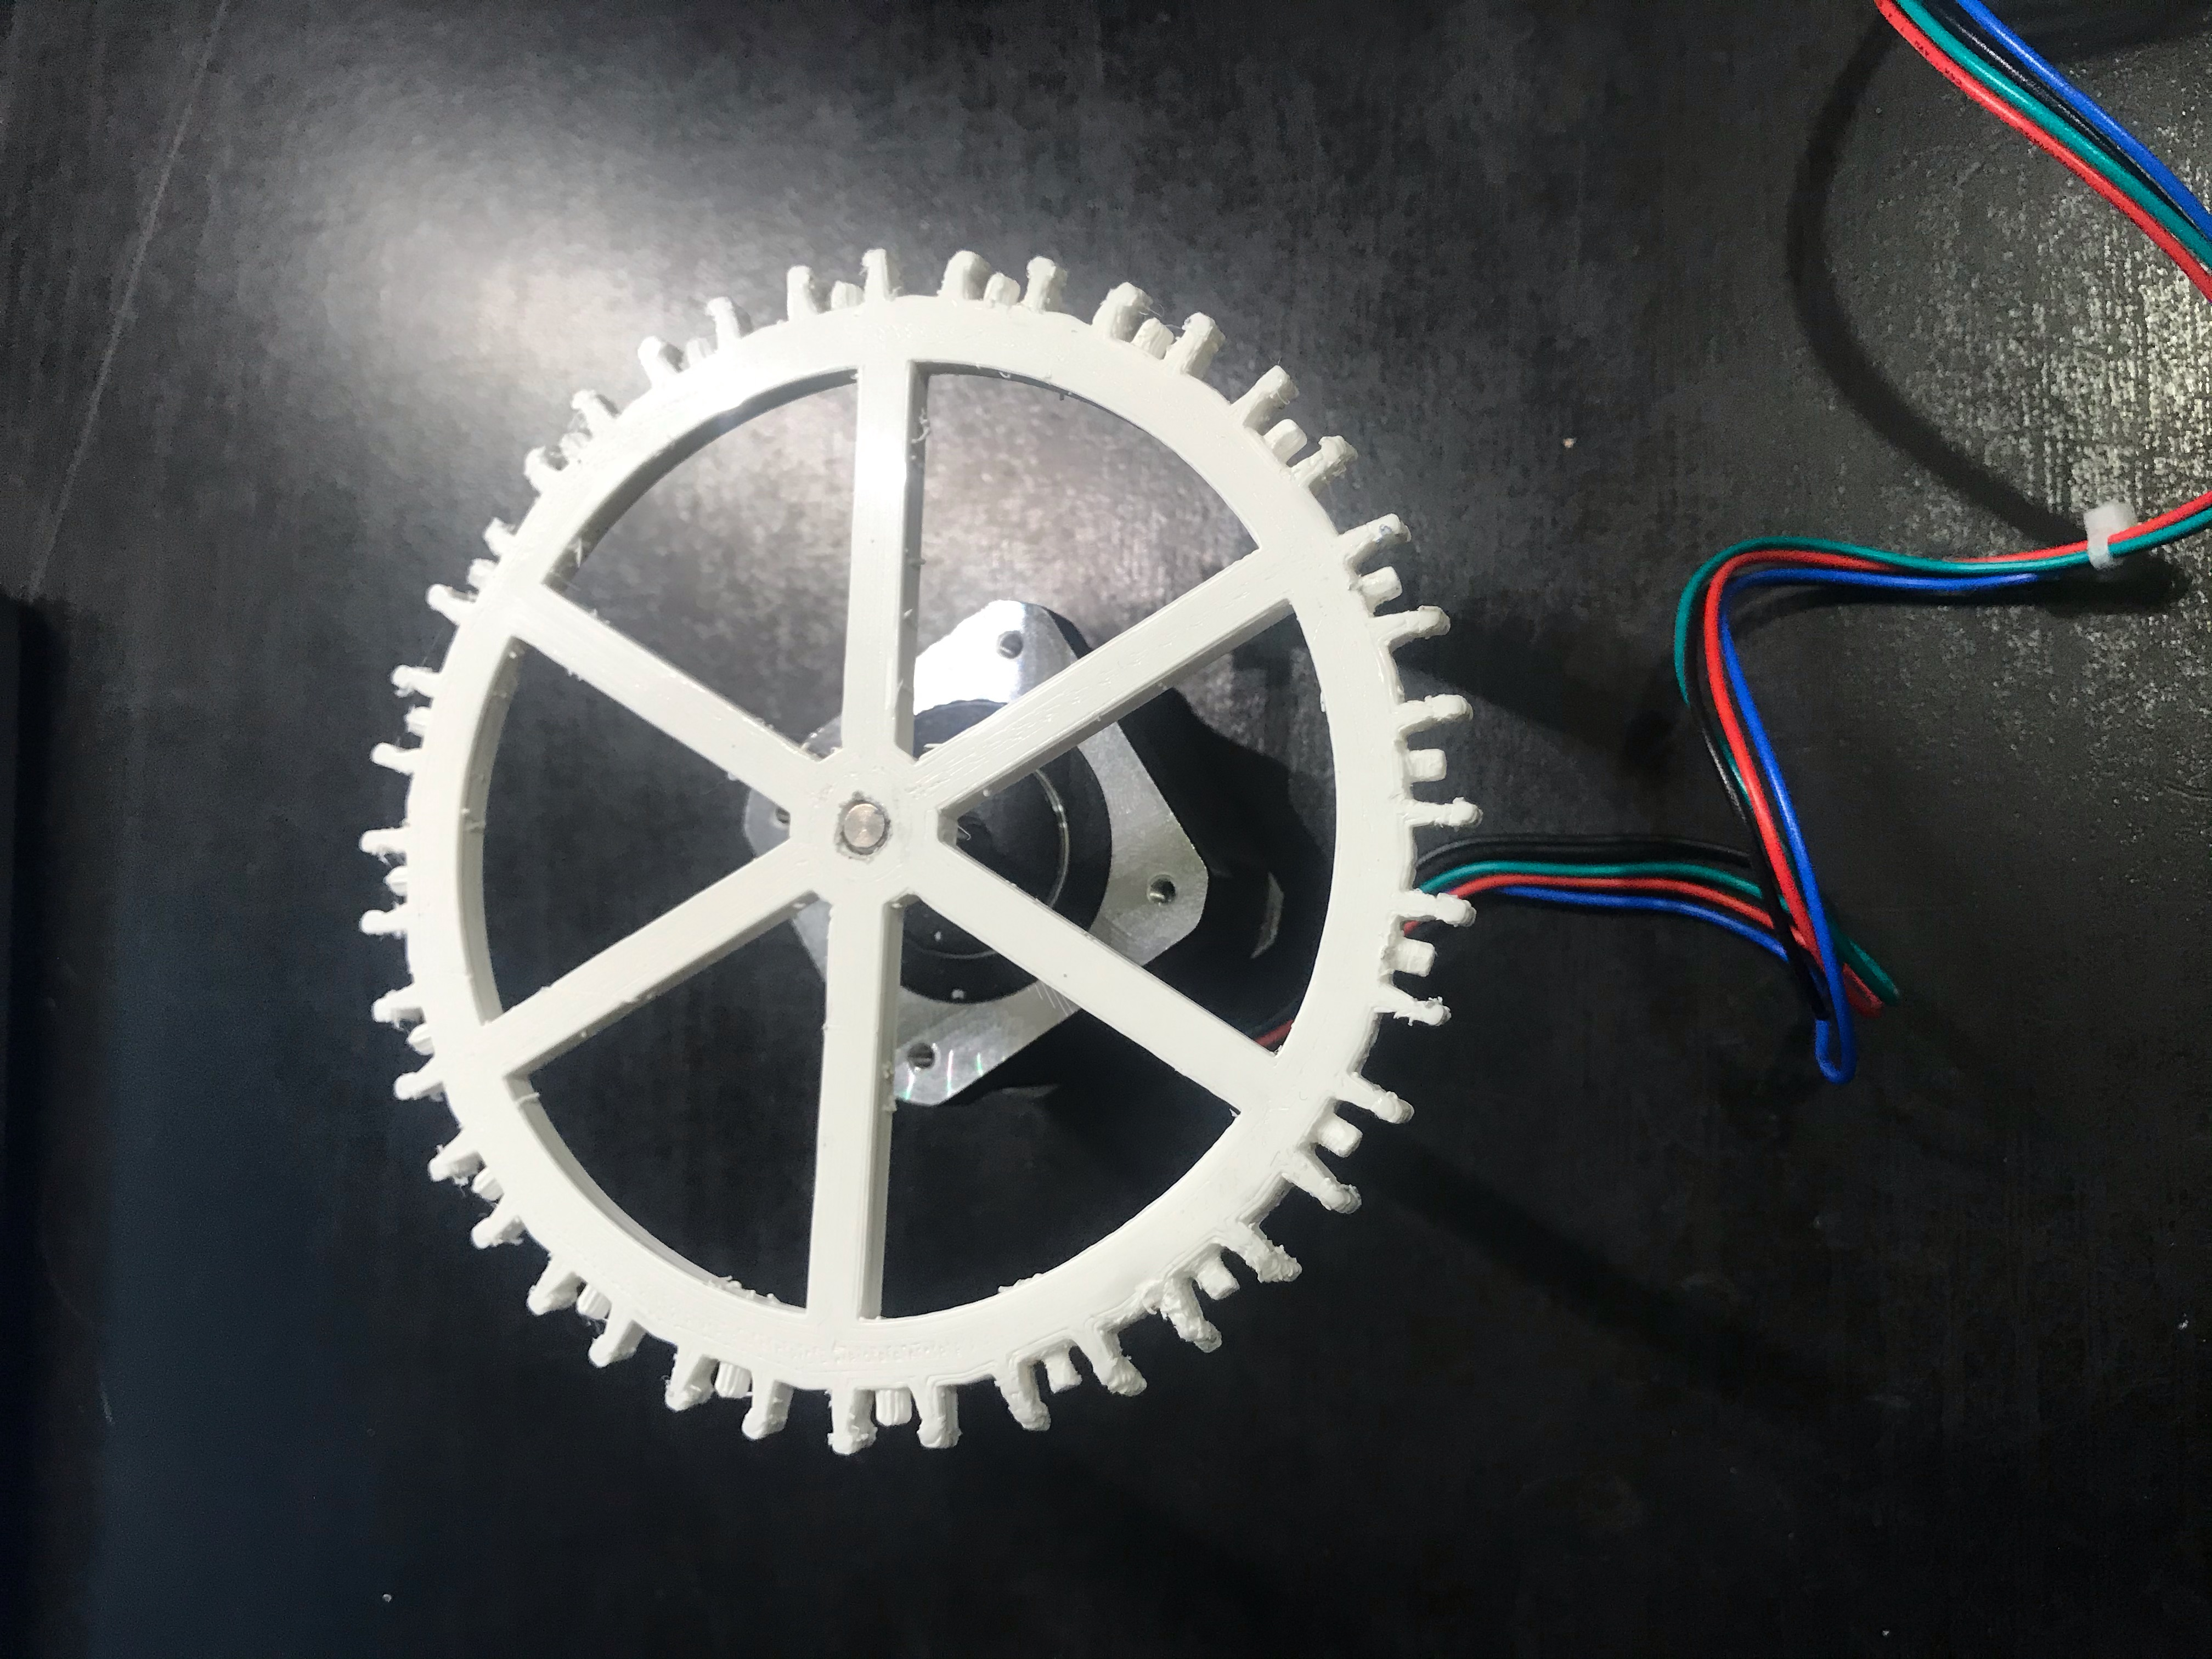
\includegraphics[height=3.125000in, keepaspectratio=true]{./first_wheel_holder/radhouder_horizontal.jpeg}



This wheel is mounted on a stepper motor with step angle of 1.8 degrees.

We can calculate the accuracy for a wheel with a radius of 5.5cm (measured to the tip of the measured tool) 

grad to radials

2*pi/360*1.8= 0.0314159265359

sin(0.031415)*55 = 1.72754081497 mm



this gives an accuracy of 1.72 mm, this is not in the accuracy range that is needed for this project. In order to get the wanted displacement per step the rotations needs to be adjusted with extra gears in the system. A displacement of less than 0.5 mm would be good.



to achieve this the calculations are made backworth:

the required angle

arcsin(0.5/55) = 0.52 degrees 

calculate how the gears should relate to each other

1.8/0.52 = 3.46153846154



round this up to 4 and recalculate the displacement per step of the motor

the angle:

1.8/4 = 0.45

2*pi/360*0.45= 0.00785398163397

sin(0.00785398163397)*55 = 0.431964548879mm



This is whithin the needed displacement range.



This needs adjustment of the current design of the wheel holder also a 3d printed footer can be printed so the wheel can circulate vertically which would make the camera and light setup easier.



\end{document}
